\documentclass[10pt,a4paper]{article} 
% Style
\usepackage{amsfonts}
\usepackage{amsmath}
\usepackage{amssymb}
\usepackage[utf8]{inputenc}
\usepackage[T1]{fontenc}
\usepackage[swedish]{babel}
\usepackage{lmodern} 
\usepackage{graphicx}
\usepackage{color}
\usepackage{float}
\usepackage{listings}
\lstset{extendedchars=\true}
\lstset{inputencoding=ansinew}
\usepackage{hyperref}

% New commands
\newcommand{\degree}{\ensuremath{^\circ}}




% Formler


% Sources

% ---Title page ---

\title{Företagsanalys Tekniska verken}

\author{Johan Berneland, johbe915\\Sofia Larsson Cahlin, sofla266\\Benjamin Lundahl, benlu392\\
    Nora Björklund, norbj648\\Christopher Hallberg, chrha007}
\date{\today}

% ---Dokument start---

\begin{document}


\maketitle

\newpage

\tableofcontents

\newpage

\section{Inledning}
Denna rapport är en del i kursen Industriell ekonomi grundkurs, TEAE01, vid Linköpings Universitet och utgörs av en analys av företaget Tekniska verken i Linköping AB, org. nr: 556004-9727.

\subsection{Bakgrund och syfte}
Syftet med denna rapport är att analysera om det valda företaget, Tekniska verken i Linköping AB, är en bra arbetsgivare. Detta sker genom att bedöma företaget främst utifrån de ekonomiska redskap och analysmetoder som getts inom ramarna för kursen. 

\subsection{Definition av bra arbetsgivare}
Vad som är en bra arbetsgivare är högst individuellt. För att kunna utföra analysen och dra slutsatser kring detta definieras här vilka aspekter som i denna rapport kännetecknar en bra arbetsgivare.

\begin{itemize}
 \item En säker anställningssituation, främst genom en stabil företagsekonomi 
 \item Bra företagsklimat
 \item Potential till personlig utveckling
 \item Marknadsanpassad ersättning
 \item Bra rykte och anseende
\end{itemize}

\section{Metod}
Rapporten grundar sig på data hämtad från årsredovisningar från företaget vad
gäller de ekonomiska delarna. I de delar som rör företagets historia, vision,
mission och liknande har vi använt oss av information från företagets hemsida.

\section{Resultat och analys}
Resultat och analys är uppdelad i tre olika avsnitt; först en beskrivning av
företaget, följt av en ekonomisk beskrivning och slutligen en SWOT-analys.

\subsection{Företagsbeskrivning}
För att kunna göra en korrekt analys av ett företag så behöver man veta vissa
grundförutsättningar. I följande avsnitt avhandlas några viktiga punkter. 

\subsubsection{Historia}
Grunden för Tekniska verken lades den 18 oktober 1902 genom startandet av
Linköpings elektriska kraft- och belysningsaktiebolag. Initiativtagare var en
entreprenör vid namn Jonn O Nilson och målet var att förse Linköpingsborna med
elström. År 1952 påbörjades fjärrvärmeutbyggnaden i Linköping och 2 år senare
kunde ett kraftvärmeverk leverera den första fjärrvärmen i Åbylund. Utbyggnaden
fortsatte och ytterligare kraftverk kom till under kommande årtionden. År 1981 
invigdes Gärstadsverket som utnyttjade avfall som bränsle. I samband med detta
började även utvecklingen för att ta till vara på avfall för att producera biogas 
och biogödsel. (Tekniska verken, 2013) 

\subsubsection{Vision, mission, affärsidé}
Tekniska verkens vision är att ''bygga världens mest resurseffektiva
region'' och deras mission är ''att tillhandahålla och utveckla
ledningsbunden infrastruktur och energilösningar för den
resurseffektiva regionen'' (Tekniska Verken ''ledning'', 2013). Det framgår även
från texter på deras hemsida att deras affärsidé är [FIXME].

\subsubsection{Ägarsituation och aktier}
Tekniska verken ägs av Linköping kommun (Tekniska verken, 2013). Deras
aktiekapital uppgår i 200 miljoner kronor och det finns 400 tusen
aktier.(Retriever, 2013)

\subsubsection{Produkter och tjänster} \label{prod}
Tekniska verken erbjuder många tjänster inom många olika sektorer i samhället.
\begin{itemize}
	\item \textbf{Energi ur avfall:} Genom att utnyttja avfall som energikälla
	produceras fjärrvärme, fjärrkyla och el till det nordiska elnätet. Dessutom och
	som följd av detta återvinner, behandlar och deponerar man avfall från hushåll
	och industrier.
	\item \textbf{Vatten:} Företaget renar vatten från sjöar och vattendrag till
	dricksvatten, renar Avloppsvatten innan det släpps ut i naturen igen, samlar
	upp nederbörd och kvalitetstestar vatten i ett laboratorium.
	\item \textbf{Infrastruktur:} Tekniska verken Driftum är en sammarbetspartner
	som tillsammans levererar kvalitativa konsulttjänster i områdena infrastruktur,
	mätteknik och energieffektivisering.
	\item \textbf{Nät:} Dotterbolaget Tekniska verken Linköping Nät AB är
	specialister på nät och förser regionen med elektricitet och bredband samt
	helhetslösningar för utomhusbelysning.
	\item \textbf{Bredband:} Tekniska verken är även delägare i bolaget Utsikt
	Bredband som är en av regionens ledande leverantörer av bredband till hushåll,
	företag, operatörer och fastighetsägare.
	\item \textbf{Miljövänlig el:} Tekniska verken är även delägare i bolaget Bixia
	AB, som köper in miljövänlig el från förnybara källor.
	\item \textbf{Biogas:} Dotterbolaget Svensk Biogas driver utvecklingen av
	marknaden för biogas och arbetar med etablering av tankställen för allmänheten.
	Dessutom utvecklar man processer och produktionskoncept.
	\item \textbf{Forskning och utveckling:} Tekniska verken arbetar även med att
	förbättra och utveckla processer som gynnar miljön och ekonomin.
\end{itemize}

\subsubsection{Marknadsstrategi och kritiska framgångsfaktorer}
Tekniska verken marknadsför sig som föregångare inom miljövänlig teknik och
effektiva energilösningar. De vill framstå som en stor och trovärdig leverantör 
av många tjänster och tekniska lösningar, som nämnts i \ref{prod}. 

%TODO Behöver kolla upp vad en KFF är. Wikipedia säger en sak och exemplet på
%lisam en annan.

\subsubsection{Marknader och marknadsandelar}
Tekniska verken är aktiva på flera olika marknader. Dessa presenteras nedan.

Avlopp:

Avfall:

El och vatten:

Värme och kyla: 

Bredband:

\subsubsection{Organisation}
Tekniska verken ägs av Linköpings kommun och ligger under Linköpings stadshus AB. Moderbolaget heter Tekniska verken i Linköping AB och har i sin tur åtta dotterbolag, främst med säten i Linköping men även i Katrineholm.  Bolagets firma tecknas av en styrelse med nio stycken ordinarie ledamöter och nio suppleanter. Den verkställande ledningen utgörs av en ledningsgrupp bestående av vd och koncernchef Anders Jonsson, vice vd, finansdirektör och olika vd:ar och chefer för vissa dotterbolag. 

Företaget har 972 anställda och i sin interna MMI-undersökning (Motiverad Medarbetar Index) från 2012 fick de 4,01 av 5. I FöretagsBarometern 2013 finns de också med på listan för Sveriges mest attraktiva arbetsgivare. 

\subsubsection{Omvärldsanalys, bransch, konkurrenter och intressenter}
Många delar av tekniska verkens verksamhetsområden ligger i områden som inte påverkas av konjunkturen i så hög grad. Det syns till exempel på rörelseresultat och vinstmarginal som inte påverkats märkvärt mellan 2007 och 2012 under vilket Sverige genomlevde lågkonjunktur (Retriever, 2013; Konj, 2013). Detta beror på att verksamheterna, till exempel vattenrening och sopsorteringen är lokala tjänster som används av invånarna i Linköpings samt omgivande kommuner och är en viktig del av 'kretsloppet' i kommunen.

Eftersom Tekniska verken är delägare i många mindre bolag finns ingen enhetlig 
bransch, utan istället många olika branscher. Företaget är på så vis verksam inom
avloppshantering, sophantering, elhandel, elproduktion, fjärrvärme, fjärrkyla, 
nätverk och bredband. Man har alltså ett mycket brett spektrum vad gäller 
verksamhetsområdet.

%TODO INSERT TEXT före intressent-biten.

De viktigaste intressenterna i Tekniska verken är, ägaren, Linköpings kommun
med dess invånare och företag. Tekniska verken är ansvariga för en rad tjänster
för kommuninvånarna, så som vatten och avlopp, avfallshantering, fjärrvärme och
elnät med mera. Vidare så är många invånare kunder till något av Tekniska
verkens dotterbolag. Exempelvis så är Bixia AB en stor el-leverantör och många
får sitt bredband genom Utsikt bredband ABs nät.

Intressenter finns även utanför kommungränserna. Cirka 25 andra kommuner
levererar avfall till Gärstad (Tekniska verken, 2013).

\subsubsection{Specifika uppförandekoder och spelregler}
Då tekniska verken arbetar i många olika branscher, måste de även ha koll på
vilka regler som gäller inom alla dessa. \\

För avfallshantering måste man uppfylla de krav som ställs av Naturvårdsverkets
som innefattar EU:s avfallsdirektiv.

För produktion av dricksvatten måste man uppfylla de krav som ställs av Riksdag
och regeringen, Livsmedelsverket, Naturvårdsverket, Havs- och Vattenmyndigheten,
Socialstyrelsen, Boverket, Kemikalieinspektionen (KemI),Strålsäkerhetsmyndigheten 
(SSM) och EU:s lagstiftning.\\

För distribuering och marknadsföring av energi i olika former så som el och
fjärrvärme, måste man rikta sig efter de krav och regler som
energimarknadsinspektionen ställer.


\subsection{Ekonomisk beskrivning}
Syftet med följande avsnitt är att få en inblick i Tekniska verkens ekonomiska
situation.

\subsubsection{Nyckeltal}
%% En massa skit, TODO: städa upp
\begin{tabular}{ l r }
	Nyckeltal & 2012-12\\
	Antal anställda, aktiebolag & 969\\
	Avkastning på eget kapital (\%) & 14,16\\
	Avkastning på totalt kapital (\%) & 6,85\\
	Skuldränta (\%) & 2,19\\
	Riskbuffert totalt kapital & 4,66\\
	Rörelseresultat före avskrivningar, EBITDA & 1 052 000\\
	Rörelsemarginal (\%) & 10,64\\
	Vinstmarginal (\%) & 10,89\\
	Omsättning per anställd & 5 410,73\\
	Soliditet (\%) & 39,39\\
	Kapitalets omsättningshastighet & 0,63\\
	Rörelsekapital & 957 000\\
	Rörelsekapital/omsättning (\%) & 18,25\\
	Kassalikviditet (\%) & 159\\
	Förändring av omsättning (\%) & -7,27\\
	Rörelseresultat per anställd & 575,85\\
	Personalkostnader per anställd & 631,58\\
	Förändring av antal anställda (\%) & -0,31\\
	Lager mm/omsättning (\%) & 2,25\\
	Kundfordringar/omsättning (\%) & 10,41\\
	Likvida medel/omsättning (\%) & 11,81\\
	Kortfristiga skulder/omsättning (\%) & 27,12\\
	Skuldsättningsgrad (\%) & 1,48\\
%%	Räntetäckningsgrad (\%) & 5,39\\
	Avkastning operativt kapital (\%) & 8,86\\
	Riskbuffert sysselsatt kapital st & 5,29\\
%%	Varulagrets omsättningshastighet & 0\\
%%	Du Pont-modellen (\%) & 6,85\\
\end{tabular}
\subsubsection{Jämförelse över tid}
Cleese löser
\begin{figure}[H] 
\centerline{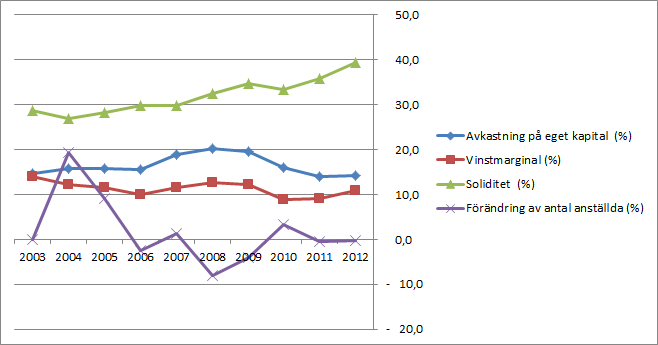
\includegraphics[scale=0.8]{Bilder/jamforelse_over_tid.png}}
\caption{Jämförelse över tid}
\end{figure}  
%% Vad ska jämföras? Nyckeltalen? Bara copy pasta från retriever?
%% Slutsatser/ren fakta?

\subsubsection{Jämförelse med konkurrenter}

\subsection{SWOT-analys}
Sofla kladdar

\subsubsection{Styrkor (Strengths)}
Hallgus skriver

\subsubsection{Svagheter (Weaknesses)}
Cleese löser

\subsubsection{Möjligheter (Opportunities)}
Benjamin


\subsubsection{Hot (Threats)}
Nora Fixar




\section{Slutsatser}

\newpage
\section{Referenser}
%% Här placeras referenser enligt Harvard metoden. Skall vara alfabetiskt, för
%% övrig info se harvard-lathunden.
%%
Tekniska verken, (2013). Avfall \& återvinning. (HTML) Tillgänglig: \\
\hyperref{http://www.tekniskaverken.se/avfall-atervinning/om/}{}{}{<http://www.tekniskaverken.se/avfall-atervinning/om/> (2013-11-27)} \\
\newline
Tekniska verken, (2013). Historiska boken. (PDF) Tillgänglig: \\
\hyperref{http://www.tekniskaverken.se/om-oss/var-historia/historiska-boken/}{}{}{<http://www.tekniskaverken.se/om-oss/var-historia/historiska-boken/> (2013-11-20)}\\
\newline
Tekniska verken, (2013). Tjänster. (HTML) Tillgänglig: \\
\hyperref{http://www.tekniskaverken.se/tjanster/}{}{}{<http://www.tekniskaverken.se/tjanster/>(2013-11-20)}\\
\newline
Retriever, (2013). Tekniska verken i Linköpping AB. (HTML) Tillgänglig: \\
\hyperref{http://web.retriever-info.com/services/businessinfo.html?method=displayBusinessInfo\&orgnum=5560049727}{}{}{<http://web.retriever-info.com/services/businessinfo.html?method=displayBu\\sinessInfo\&orgnum=5560049727> (2013-12-04)}\\
\newline
Konj, (2013). Konjunkturläget juni 2013. (PDF) Tillgänglig:\\
\hyperref{http://www.konj.se/download/18.6a90e2ce13e070b080d1a1f/Konjunkturl\%C3\%A4get+juni+2013.pdf}{}{}{<http://www.konj.se/download/18.6a90e2ce13e070b080d1a1f/Konjunkturl\%C\\3\%A4get+juni+2013.pdf> (2013-12-04)}\\
\newline
Svenskt Vatten, (2013). Dricksvatten. (HTML) Tillgänglig: \\
\hyperref{http://www.svensktvatten.se/Vattentjanster/Dricksvatten/Lagar-och-foreskrifter/}{}{}{<http://www.svensktvatten.se/Vattentjanster/Dricksvatten/Lagar-och-foreskrifter/>
(2013-11-20)} \\
\newline
Naturvårdsverket, (2013). Avfallshantering. (HTML) Tillgänglig: \\
\hyperref{http://www.naturvardsverket.se/Stod-i-miljoarbetet/Vagledning-amnesvis/Avfall/Lagar-och-regler-om-avfall/}{}{}{http://www.naturvardsverket.se/Stod-i-miljoarbetet/Vagledning-amnesvis/Avfall/Lagar-och-regler-om-avfall/(2013-11-20)}\\
\newline
Energimarknadsinspektionen, (2013). Avfallshantering. (HTML) Tillgänglig: \\
\hyperref{http://www.energimarknadsinspektionen.se/sv/el/}{}{}{http://www.energimarknadsinspektionen.se/sv/el/(2013-11-20)}\\

\end{document}



%%% Local Variables: 
%%% TeX-PDF-mode: t 
%%% TeX-master: "rapport"
%%% End: 

